\section{DIDA 理论分析}
\label{sec:th_analysis_imitation}

本节理论分析旨在实现两个目标。
首先，为延迟策略与无延迟策略之间的性能差异提供界。
这些界将依赖于环境平滑性假设（见\cref{{subsec:smooth_mdp}}）。
其次，研究这些界有助于理解哪些无延迟专家更适于在延迟环境中被模仿。


\subsection{延迟与无延迟性能的比较}
\label{subsec:compare_delayed_undelayed}

在直接给出理论结果之前，有必要澄清一点。
需要比较延迟策略和无延迟策略的价值函数，然而它们的输入空间不同。
具体而言，延迟策略 $\delayedpolicy$ 的输入空间为 $\augmentedstatespace=\statespace\times\actionspace^\delay$，而无延迟策略的输入空间为 $\statespace$。
下文详述文献中提出的两种比较方式。

\subsubsection{弱随机马尔可夫决策过程中的比较}
比较延迟策略与无延迟策略的一种可能方式由 \cite{walsh2009learning} 提出。
其思想源于以下观察：若 \gls{dmdp} 源自确定性 \gls{mdp}，则它们有相同的最优性能（直到\Cref{subsec:delay_init} 中提到的延迟初始化偏移）。
这易于理解：利用环境的确定性模型计算当前状态后，智能体可选择无延迟策略在该状态下推荐的动作。显然，困难在于学习 \gls{mdp} 的模型。
为扩展这一比较，\cite{walsh2009learning} 考虑了所谓的弱随机（mildly stochastic）\gls{mdp}，即满足如下条件的 \gls{mdp}：
\begin{align*}
    \exists \epsilon \text{ s.t. } \forall (s,a)\in\statespace\times\actionspace, \exists s', p(s'\vert s,a)\geq 1-\epsilon.
\end{align*}
由于这些 \glspl{mdp} 仅是弱随机的，可按上述方式针对 \gls{mdp} 的确定性近似学习最优延迟策略。
记 $\widehat{V}^{\pi}$ 为无延迟策略在 \gls{mdp} 确定性近似中的价值函数，则有 \cite[Theorem~3]{walsh2009learning}：
\begin{align*}
    \lVert \widehat{V}^{\pi}-{V}^{\pi}\rVert_{\infty}\leq \frac{\gamma\epsilon \maximumreward}{(1-\gamma)^2},
\end{align*}
其中 ${V}^{\pi}$ 是同一策略 $\pi$ 在无延迟 \gls{mdp} 中的价值函数。
注意这两个价值函数的输入空间均为 $\statespace$。
另一个值得注意的观察是，结果对有效时域 $\textstyle\frac{1}{1-\gamma}$ 呈二次依赖关系。
弱随机性假设相当强，本文将为更弱的假设提供结果。

\subsubsection{基于信念分布的比较}
另一种方法的优势在于可适用于任意 \gls{mdp}，由 \cite{agarwal2021blind} 提出。
对于给定增广状态 $x\in\augmentedstatespace$，作者比较了延迟策略的价值函数 $V^{\delayedpolicy}(x)$ 与无延迟策略在给定 $x$ 下信念的期望价值函数 $\textstyle\expectedvalue_{s\sim \augmentedbelief(\cdot\vert x)}[V^{\pi}(s)]$。
作者提出学习一种延迟策略，该策略选择的动作最大化无延迟策略 Q 函数在信念分布下的期望。
假设动作空间基数有限 $\cardinal{\actionspace}$，延迟策略 $\delayedpolicy$ 相对于最优策略 $\optimalpolicy$ 具有如下保证 \cite[Theorem~1]{agarwal2021blind}：
\begin{align*}
    V^\delayedpolicy(x) \ge \expectedvalue_{s\sim \augmentedbelief(\cdot\vert x)}[V^{\optimalpolicy}(s)] - \frac{\maximumreward}{(1-\gamma)^2}\left(1-\frac{1}{\cardinal{\actionspace}}\right)
\end{align*}
再次注意对有效时域的二次依赖关系。
在本文的分析中，将比较相同量，同时增加对底层 \gls{mdp} 平滑性的假设。




\subsection{常值延迟性能损失的上界}
\label{subsec:imitation_upper_bound}
在理论部分的余下内容中，假设底层 \gls{mdp} 是平滑的。具体而言，需要 \gls{mdp} 是 $(L_P,L_r)$-LC 的（见\Cref{def:lip_mdp}），且专家的无延迟策略是 $L_\pi$-LC 的（见\Cref{def:lip_policy}）。
此外，还需要其 Q 函数是 $L_Q$-LC 的\footnote{在某些情形下，这可由前两个假设推出，见\Cref{th:lip_Q_function}。}。
这些平滑性保证的优点在于排除了诸如\Cref{pp:counter_example_belief_based} 中的病态例子。
然而，该设定仍然是现实的，因为许多物理系统是 Lipschitz 的。

为给出上界的主要结果，首先推导延迟情形下性能差异引理~\cite[Lemma~6.1]{kakade2002approximately} 的改编版本。
该结果本身可能对延迟文献有用。
该结果曾在 \cite[Equation~32]{agarwal2021blind} 中针对整数延迟独立推导，但本文给出一个更通用的版本，适用于延迟 $\delay\in\realnumbers[\ge0]$。
下文中，记 $\discountedstateoccupancydistribution[x][\delayedpolicy]$ 为延迟策略 $\delayedpolicy$ 从增广状态 $x$ 出发在增广状态空间 $\augmentedstatespace$ 上的折扣状态占据分布。


\begin{lemma}
[延迟性能差异引理（Delayed Performance Difference Lemma）]
\label{lem:perf_diff_lem}
    对于某些 $\delay\in\realnumbers[\ge0]$，设 $\pi$ 为无延迟策略，$\delayedpolicy$ 为同一底层 \gls{mdp} $\markovdecisionprocess$ 上的 $\delay$-延迟策略。
    则 $\forall x\in\mathcal{X}$，
    \begin{align*}
        \expectedvalue_{s\sim \augmentedbelief(\cdot\vert x)}[V^{\pi}(s)] - V^{\delayedpolicy}(x)
        = \frac{1}{1-\gamma}
        \quad\expectedvalue_{x'\sim \delayeddiscountedstateoccupancydistribution[x][\delayedpolicy]} \left[ \expectedvalue_{s\sim \augmentedbelief(\cdot\vert x')}[V^{\pi}(s)] -  \expectedvalue_{\substack{s\sim \augmentedbelief(\cdot\vert x')\\a\sim \delayedpolicy(\cdot\vert x')}}[Q^{\pi}(s,a)] \right].
    \end{align*}
\end{lemma}
\begin{proof}
    首先证明整数延迟下的结果。

    \noindent\textbf{整数延迟。}\indent 考虑 $\delay\in\naturalnumbers$，$x\in\augmentedstatespace$，设
    \begin{align*}
        I(x)=\expectedvalue_{s\sim \augmentedbelief(\cdot\vert x)}[V^{\pi}(s)] - V^{\delayedpolicy}(x).
    \end{align*}
    通过对 $I$ 加上并减去同一量，得到：
    \begin{align*}
        I(x)
        &= \underbrace{\expectedvalue_{s\sim \augmentedbelief(\cdot\vert x)}[V^{\pi}(s)] - \expectedvalue_{\substack{s\sim \augmentedbelief(\cdot\vert x)\\a\sim \delayedpolicy(\cdot\vert x)}}\left[r(s,a) + \gamma \expectedvalue_{s'\sim p(\cdot\vert s,a)}[V^{\pi}(s')]\right]}_{\eqcolon A}
        \\
        &\quad + \underbrace{\expectedvalue_{\substack{s\sim \augmentedbelief(\cdot\vert x)\\a\sim \delayedpolicy(\cdot\vert x)}}\left[r(s,a) + \gamma \expectedvalue_{s'\sim p(\cdot\vert s,a)}[V^{\pi}(s')]\right] - V^{\delayedpolicy}(x)}_{\eqcolon B}.
    \end{align*}
    然后分析上式中的每一项。首先，
    \begin{align*}
        A = \expectedvalue_{s\sim \augmentedbelief(\cdot\vert x)}[V^{\pi}(s)] - \expectedvalue_{\substack{s\sim \augmentedbelief(\cdot\vert x)\\a\sim \delayedpolicy(\cdot\vert x)}}\left[Q^{\pi}(s,a)\right].
    \end{align*}
    其次，由于 $V^{\delayedpolicy}(x) = \expectedvalue_{\substack{s\sim \augmentedbelief(\cdot\vert x)\\a\sim \delayedpolicy(\cdot\vert x)}}\left[r(s,a)\right]+ \gamma \expectedvalue_{\substack{x'\sim \augmentedtransitionfunction(\cdot\vert x,a)\\a\sim \delayedpolicy(\cdot\vert x)}}[V^{\delayedpolicy}(x')]$，则，
    \begin{align*}
        B &= \gamma\expectedvalue_{\substack{s\sim \augmentedbelief(\cdot\vert x)\\a\sim \delayedpolicy(\cdot\vert x)}}\left[ \expectedvalue_{s'\sim p(\cdot\vert s,a)}[V^{\pi}(s')]\right] - \gamma \expectedvalue_{\substack{x'\sim \augmentedtransitionfunction(\cdot\vert x,a)\\a\sim \delayedpolicy(\cdot\vert x)}}[V^{\delayedpolicy}(x')].
    \end{align*}
    注意，
    \begin{align}
    \label{eq:perf_diff_lem_equiv_belief}
        \int_{\statespace} \augmentedbelief(s\vert x)p(s'\vert s,a)\de s = \int_{\augmentedstatespace}\augmentedtransitionfunction(x'\vert x,a)\augmentedbelief(s'\vert x')\de x'.
    \end{align}
    这意味着，给定当前增广状态 $x$ 和某动作 $a$，下一个未观测当前状态为 $s'$ 的概率可通过两种方式获得：要么先以当前未观测状态 $s$ 为条件，要么以下一个增广状态 $x'$ 为条件。
    由此得到，
    \begin{align*}
        B &= \gamma \expectedvalue_{\substack{x'\sim \augmentedtransitionfunction(\cdot\vert x,a)\\a\sim \delayedpolicy(\cdot\vert x)}}\left[\expectedvalue_{s\sim \augmentedbelief(\cdot\vert x')}[V^{\pi}(s')] - V^{\delayedpolicy}(x') \right]
        \\
        &= \gamma \expectedvalue_{\substack{x'\sim \augmentedtransitionfunction(\cdot\vert x,a)\\a\sim \delayedpolicy(\cdot\vert x)}}\left[I(x')\right],
    \end{align*}
    通过识别量 $I$。现在，如同原始引理，迭代此结果：
    \begin{align}
        I(x) &= \sum_{t=0}^\infty \gamma^t \expectedvalue_{\substack{x_{t+1}\sim \augmentedtransitionfunction(\cdot\vert x_t,a_t)\\a_t\sim \delayedpolicy(\cdot\vert x_t)}}\left[\left. \expectedvalue_{s\sim \augmentedbelief(\cdot\vert x_t)}[V^{\pi}(s)] - \expectedvalue_{\substack{s\sim \augmentedbelief(\cdot\vert x_t)\\a\sim \delayedpolicy(\cdot\vert x_t)}}[Q^{\pi}(s,a)] \right\vert x_0=x \right]\nonumber
        \\
        &= \frac{1}{1-\gamma}\expectedvalue_{x'\sim \delayeddiscountedstateoccupancydistribution[x][\delayedpolicy]}\left[ \expectedvalue_{s\sim \augmentedbelief(\cdot\vert x')}[V^{\pi}(s)] - \expectedvalue_{\substack{s\sim \augmentedbelief(\cdot\vert x')\\a\sim \delayedpolicy(\cdot\vert x')}}[Q^{\pi}(s,a)] \right],\label{eq:state_distrib_reco}
    \end{align}
    其中\Cref{eq:state_distrib_reco} 由策略 $\delayedpolicy$ 的折扣增广状态占据分布定义得到（见\Cref{def:discounted_state_distrib}）。
    因此，证明了 $\delay\in\naturalnumbers$ 下的结果。

    \noindent\textbf{非整数延迟。}\indent 为证明清晰起见，假设 $\delay\in(0,1)$，但 $\delay\in\realnumbers[\ge0]$ 的一般结果可由此轻松导出。
    注意此时信念的定义如\Cref{subsec:non_int_delays} 所示。
    前述整数延迟的证明可顺利应用于非整数延迟。
    唯一可能不易直接推导的步骤是\Cref{eq:perf_diff_lem_equiv_belief}。
    因此，下面详述该步骤。
    对于 $x_t=(s_t,a_{t-1}), x_{t+1}=(s_{t+1},a_t)\in\augmentedstatespace$，
    \begin{align}
        &\int_{\statespace} \augmentedbelief(s_{t+\delay}\vert x_t)p(s_{t+1+\delay}\vert s_{t+\delay},a)\de s_{t+\delay}\nonumber
        \\
        &\qquad=\int_{\statespace} \augmentedbelief(s_{t+\delay}\vert x_t) \int_{\statespace}  \augmentedbelief(s_{t+1+\delay}\vert s_{t+1},a) b_{1-\delay}(s_{t+1}\vert s_{t+\delay},a)\de s_{t+1}\de s_{t+\delay} \label{eq:use_def_p_non_int}
        \\
        &\qquad= \int_{\statespace} \augmentedbelief(s_{t+1+\delay}\vert s_{t+1},a)\int_{\statespace} \augmentedbelief(s_{t+\delay}\vert x_t)b_{1-\delay}(s_{t+1}\vert s_{t+\delay},a)\de s_{t+\delay}\de s_{t+1} \nonumber
        \\
        &\qquad= \int_{\statespace} \augmentedbelief(s_{t+1+\delay}\vert s_{t+1},a)\int_{\statespace} \augmentedbelief(s_{t+\delay}\vert s_t,a_{t-1})b_{1-\delay}(s_{t+1}\vert s_{t+\delay},a)\de s_{t+\delay}\de s_{t+1} \nonumber
        \\
        &\qquad= \int_{\actionspace} \int_{\statespace} \augmentedbelief(s_{t+1+\delay}\vert s_{t+1},a_{t}) \delta_{a}(a_{t})\nonumber
        \\
        &\qquad\quad\int_{\statespace} \augmentedbelief(s_{t+\delay}\vert s_t,a_{t-1}) b_{1-\delay}(s_{t+1}\vert s_{t+\delay},a)\de s_{t+\delay}\de s_{t+1}\de a_{t}\nonumber
        \\
        &\qquad= \int_\augmentedstatespace \augmentedbelief(s_{t+1+\delay}\vert x_{t+1})\tilde p(x_{t+1}\vert x_t, a)\de x_{t+1}\label{eq:def_aug_mdp_p_non_int}.
    \end{align}
    \Cref{eq:use_def_p_non_int} 由\Cref{eq:def_p_non_int} 中 $p$ 的定义得到，\Cref{eq:def_aug_mdp_p_non_int} 通过识别增广 \gls{mdp} 中的转移得到。
\end{proof}


下面陈述本章的主要结果。
该结果不仅对 DIDA 有价值，对任何满足\Cref{eq:belief_pol} 的策略均有价值。
\glspl{dmdp} 的平滑性是证明的关键要素。

\begin{thm}
\label{th:perf_diff_bound}
    设 $\markovdecisionprocess$ 是 $(L_P,L_r)$-LC 的 \gls{mdp}，$\pi$ 是 $L_\pi$-LC 的无延迟策略。进一步假设 $Q^{\pi}$ 是 $L_Q$-LC 的\footnote{证明仅需 $Q^{\pi}$ 在第二个参数上的 Lipschitz 性质。}。
    设 $\delay\in\realnumbers[\ge0]$，并考虑满足\Cref{eq:belief_pol} 的 $\delay$-延迟策略 $\delayedpolicy$。
    则 $\forall x\in\mathcal{X}$，
    \begin{align*}
        \expectedvalue_{s\sim \augmentedbelief(\cdot\vert x)}&[V^{\pi}(s)] - V^{\delayedpolicy}(x) \leq \frac{L_Q L_\pi}{1-\gamma} \sigma_b^x,
    \end{align*}
    其中
    \begin{align*}
        \sigma_b^x = \expectedvalue_{\substack{x'\sim \delayeddiscountedstateoccupancydistribution[x][\delayedpolicy]\\ s,s'\sim \augmentedbelief(\cdot\vert x')}}\left[ \distance_{\statespace}(s,s') \right].
    \end{align*}
\end{thm}
\begin{proof}
    本证明无需区分整数和非整数延迟。
    设 $\delay\in\realnumbers[\ge0]$。由\Cref{lem:perf_diff_lem}，对于某些 $x \in \augmentedstatespace$，
    \begin{align*}
        \expectedvalue_{s\sim \augmentedbelief(\cdot\vert x)}&[V^{\pi}(s)] - V^{\delayedpolicy}(x)
        = \frac{1}{1-\gamma} \expectedvalue_{x'\sim \delayeddiscountedstateoccupancydistribution[x][\delayedpolicy]} \bigg[\underbrace{ \expectedvalue_{s\sim \augmentedbelief(\cdot\vert x')}[V^{\pi}(s)] -  \expectedvalue_{\substack{s\sim \augmentedbelief(\cdot\vert x')\\a\sim \delayedpolicy(\cdot\vert x')}}[Q^{\pi}(s,a)]}_{A(x')} \bigg].
    \end{align*}
    关注项 $A(x')$。有，
    \begin{align}
        A(x')
        &= \expectedvalue_{s\sim \augmentedbelief(\cdot\vert x')}\left[\expectedvalue_{\substack{a_1\sim\pi(\cdot\vert s) \\a_2\sim \delayedpolicy(\cdot\vert x')}}\left[ Q^{\pi}(s,a_1) -  Q^{\pi}(s,a_2) \right]\right]\nonumber
        \\
        &\leq L_Q \expectedvalue_{s\sim \augmentedbelief(\cdot\vert x')} \left[ \wassersteindistance(\pi(\cdot\vert s)
        \Vert \delayedpolicy(\cdot\vert x') ) \right],\label{eq:partial_res_v}
    \end{align}
    其中结果由应用\Cref{pp:expected_q_bound} 得到。
    最后一步是使用 $\sigma_b^x$ 对
    $\expectedvalue_{s\sim \augmentedbelief(\cdot\vert x')} \left[ \wassersteindistance(\pi(\cdot\vert s) \Vert \delayedpolicy(\cdot\vert x') ) \right]$ 进行上界估计。因此，
    \begin{align}
         \wassersteindistance(\pi(\cdot\vert s) \Vert \delayedpolicy(\cdot\vert x') )
        &= \sup_{\left\Vert f\right\Vert_L\leq 1}\left\vert\int_{\actionspace} f(a)(\pi(a\vert s)-\delayedpolicy(a\vert x')) \de a\right\vert \nonumber
        \\
        &= \sup_{\left\Vert f\right\Vert_L\leq 1}\left\vert\int_{\actionspace} f(a)(\pi(a\vert s)-\int_{\statespace}\pi(a\vert s')\augmentedbelief(s'\vert x')\de s') \de a\right\vert \label{eq:def_pidel}
        \\
        &\leq  \int_{\statespace} \augmentedbelief(s'\vert x') \sup_{\left\Vert f\right\Vert_L\leq 1}\left\vert\int_{\actionspace} f(a)(\pi(a\vert s)-\pi(a\vert s')) \de a \right\vert \de s' \label{eq:fub_ton_sigma}
        \\
        &\leq \int_{\statespace} \augmentedbelief(s'\vert x') \wassersteindistance(\pi(\cdot\vert s) \Vert \pi(\cdot\vert s') ) \de s'\nonumber
        \\
        &\leq L_\pi \int_{\statespace} \augmentedbelief(s'\vert x')  \distance_{\statespace}(s,s') \de s'
        \label{eq:lip_expert_pol}
        ,
    \end{align}
    其中\Cref{eq:def_pidel} 由\Cref{eq:belief_pol} 得到，\Cref{eq:fub_ton_sigma} 由 Fubini-Tonelli 定理得到，\Cref{eq:lip_expert_pol} 由 $\pi$ 的 Lipschitz 性质得到。
    将此结果代入\Cref{eq:partial_res_v} 即得结论。
\end{proof}

为使该结果更具实际解释性，提供两种方式进一步约束非常见项 $\sigma_b^x$，每种方式引入一个新的假设。
第一个结果假设 \gls{mdp} 具有时间 Lipschitz 性质（见\Cref{def:time_lip}）。

\begin{coroll}
\label{cor:perf_diff_bound_tlc}
    若\Cref{th:perf_diff_bound} 的假设成立，且此外 \gls{mdp} 是 $L_T$-TLC 的，则 $\forall x\in\mathcal{X}$，
    \begin{align*}
        \expectedvalue_{s\sim \augmentedbelief(\cdot\vert x)}&[V^{\pi}(s)] - V^{\delayedpolicy}(x) \leq \frac{2 \delay L_T L_Q L_\pi}{1-\gamma}.
    \end{align*}
\end{coroll}
\begin{proof}
    将\Cref{lem:bound_sigma_tlc} 应用于\Cref{th:perf_diff_bound} 即得结果。
\end{proof}

该结果清晰表明，性能差异的界与延迟呈线性关系。
该界的一个关键局限性在于，当 \gls{mdp} 变为确定性时，它不会趋于 0。事实上，如\Cref{subsec:compare_delayed_undelayed} 所述，在这种情况下，最优延迟回报应与无延迟回报匹配。
下面给出的 \Cref{th:perf_diff_bound} 的第二个推论则没有这一局限性。

\begin{coroll}
\label{cor:perf_diff_bound_eucl}
    若\Cref{th:perf_diff_bound} 的假设成立，且此外 $\statespace\subseteq\realnumbers^n$ 配备欧几里得范数，则 $\forall x\in\mathcal{X}$，
    \begin{align*}
        \expectedvalue_{s\sim \augmentedbelief(\cdot\vert x)}[V^{\pi}(s)] - V^{\delayedpolicy}(x) \leq
        \frac{\sqrt{2} L_Q L_\pi}{1-\gamma}
        \expectedvalue_{x'\sim \delayeddiscountedstateoccupancydistribution[x][\delayedpolicy]}\left[\sqrt{ \variance_{s\sim \augmentedbelief(\cdot\vert x')}(s\vert x')}\right].
    \end{align*}
\end{coroll}
\begin{proof}
    将\Cref{lem:bound_sigma_eucl} 应用于\Cref{th:perf_diff_bound} 即得结果。
\end{proof}

为评估这些界的质量，下面给出性能差异的下界结果。


\subsection{常值延迟性能损失的下界}
本小节通过展示在相同平滑性假设下，当专家的无延迟策略为最优时，\Cref{cor:perf_diff_bound_eucl} 与一个下界在常数项内匹配，从而增加其意义。

\begin{thm}
\label{th:lb_tight}
设 $L_\pi>0$，$L_{Q}>0$，$\delay\in\realnumbers[\ge0]$。
则存在一个 \gls{mdp}，其最优 $L_\pi$-LC 策略 $\optimalpolicy$ 的价值函数在第二个参数上是 $L_{Q}$-LC 的，但对任意 $\delay$-延迟策略 $\delayedpolicy$ 和 $x\in\augmentedstatespace$，
    \begin{align*}
        \expectedvalue_{s\sim \augmentedbelief(\cdot\vert x)}[\optimalstatevaluefunction(s)] - V^{\delayedpolicy}(x) &\geq
        \frac{\sqrt 2}{\sqrt \pi}\frac{ L_{Q}L_\pi}{1-\gamma}
        \expectedvalue_{x'\sim \delayeddiscountedstateoccupancydistribution[x][\delayedpolicy]}\left[\sqrt{ \variance_{s\sim \augmentedbelief(\cdot|x')}(s|x')}\right],
    \end{align*}
    其中 $\optimalstatevaluefunction$ 为最优无延迟策略的价值函数。
\end{thm}
\begin{proof}
    对于给定的 $L_\pi>0$，$L_{Q}>0$ 和 $\delay\in\realnumbers[\ge0]$，设计一个 \gls{mdp} $\markovdecisionprocess=(\statespace,\actionspace, \transitionfunction, \rewardfunction, \initialstatedistribution)$ 使得：$\statespace=\realnumbers$；$\actionspace=\realnumbers$；其转移函数为
    \begin{align*}
        \transitionfunction(s'\vert s,a)=\mathcal N\left(s';\; s+\frac{a}{L_\pi},\sigma^2\right),
    \end{align*}
    即 $s'=s+\frac{a}{L_\pi}+\varepsilon$，其中 $\varepsilon \sim \mathcal N (0,\sigma^2)$；
    其奖励函数为
    \begin{align*}
        \expectedrewardfunction(s,a)=\expectedvalue[\rewardfunction(s,a)] = -L_r\left\vert s+\frac{a}{L_\pi}\right\vert,
    \end{align*}
    其中 $L_r:=L_Q L_\pi$。
    在 $\expectedrewardfunction$ 的定义中使用 $L_Q$，因为后文将证明这正是 $\optimalstateactionvaluefunction$ 的 Lipschitz 常数。
    注意 $\forall (s,a)\in\statespace\times\actionspace,\;r(s,a)\le0$，但策略 $\optimalpolicy(a\vert s)=\delta_{-L_\pi s}(a)$ 对任意状态-动作对 $(s,a)$ 获得奖励 $0$。
    这意味着 $\optimalstatevaluefunction=0$ 处处成立。

    现在证明 Q 函数是 Lipschitz 的，
    \begin{align*}
        \optimalstateactionvaluefunction(s,a)&=-L_r\left\vert s+\frac{a}{L_\pi}\right\vert + \gamma \int_{\realnumbers} \optimalstatevaluefunction(s')\ p(s'\vert s,a)\de s'
        \\
        &= -L_r\left\vert s+\frac{a}{L_\pi}\right\vert
        \\
        &=-L_{Q}\left\vert L_\pi s+a\right\vert.
    \end{align*}
    因此，$\optimalstateactionvaluefunction$ 在第二个参数上是 $L_Q$-LC 的。

    现在研究 $\delay$-延迟策略 $\delayedpolicy$ 的情形。
    对于给定时间步 $t$，未观测当前状态为
    \begin{align*}
        s_t=\underbrace{s_{t-\delay}+\sum_{\tau=t-\delay}^{t-1} \frac{a_\tau}{L_\pi}}_{\eqqcolon \phi(x_t)}+\underbrace{\sum_{\tau=t-\delay}^{t-1} \varepsilon_\tau}_{\eqqcolon\epsilon}.
    \end{align*}
    上面定义了两个量。第一个 $\phi(x_t)$ 是增广状态 $x_t\in\augmentedstatespace$ 的确定性函数。
    第二个 $\epsilon$ 是服从分布 $\mathcal N(0,\delay\sigma^2)$ 的随机变量。
    利用这些量，可以定义增广奖励为，
    \begin{align*}
        \augmentedexpectedrewardfunction (x_t,a)
        &= -L_r\expectedvalue\left[\Big\vert s_t+\frac{a}{L_\pi}\Big\vert\right]
        \\
        &=-L_r\expectedvalue\left[\Big\vert\phi(x_t)+\frac{a}{L_\pi}+\epsilon\Big\vert\right].
    \end{align*}
    因此奖励正比于函数 $f:a\mapsto\expectedvalue\left[\left\vert \mathcal N(g(a),\delay\sigma)\right\vert\right]$，其中 $\textstyle g(a)=\phi(x_t)+\frac{a}{L_\pi}$。$f$ 的最小值在 $g(a)=0$ 处取得，对应于半正态分布的均值，即 $\textstyle\min_{a\in\realnumbers}f(a)=\frac{\sigma\sqrt{2\delay}}{\sqrt{\pi}}$，因此，
    \begin{align*}
        \augmentedexpectedrewardfunction (x_t,a)
        &\le -{L_r}\frac{\sqrt {2\delay}}{\sqrt \pi}\sigma.
    \end{align*}
    于是，
    \begin{align*}
        V^{\delayedpolicy}(x)
        &= \expectedvalue_{\substack{x_{t+1}\sim\augmentedtransitionfunction(\cdot\vert x_t,a_t)\\a_t\sim\delayedpolicy(\cdot\vert s_t)}} \left[\left.\sum_{t=0}^\infty \gamma^t \augmentedexpectedrewardfunction(x_t,a_t)\right\vert x_0=x\right]
        \\
        &\leq-\frac{L_r}{1-\gamma}\frac{\sqrt {2\delay}}{\sqrt \pi}\sigma
        \\
        &= -\frac{L_Q L_\pi}{1-\gamma}\frac{\sqrt {2}}{\sqrt \pi}\expectedvalue_{x'\sim \delayeddiscountedstateoccupancydistribution[x][\delayedpolicy]}\left[\sqrt{ \variance_{s\sim \augmentedbelief(\cdot|x')}(s|x')}\right],
    \end{align*}
    其中，第一个不等式中注意到，根据 $\markovdecisionprocess$ 的定义，任何未观测当前状态的方差相同。
    最后一个不等式中，将 $L_r$ 替换为 $L_Q L_\pi$，将 $\delay\sigma^2$ 替换为信念上的方差 $\mathbb Var_{s\sim b(\cdot\vert x)}(s\vert x)$。
    该不等式与 $\optimalstatevaluefunction=0$ 在任意状态成立的事实共同完成了证明。
\end{proof}

该结果凸显出专家的策略越粗糙，保证越弱。

\subsection{常值延迟的启示}
下面讨论前述理论结果的含义。
这些界在策略 $\delayedpolicy$ 完美模仿了无延迟策略且满足\Cref{eq:belief_pol} 时成立。
实践中可能并非如此，这是性能损失的第一来源。
性能损失的第二个来源是无延迟策略本身可能并非最优，虽然这不影响界，但会降低智能体的最终性能。

特别指出两个关键权衡。
首先，更平滑的专家在无延迟环境中可能是次优的，但根据\Cref{th:perf_diff_bound}，这为延迟策略提供了更简单的模仿问题。
其次，更嘈杂的策略在无延迟环境中也可能次优，但通过提供错误决策及如何从中恢复的示例，可以简化模仿任务~\cite{laskey2017dart}。



\subsection{随机延迟性能损失的界}
\label{subsec:stoch_delay_dida}
本小节研究将 DIDA 应用于随机整数延迟时的保证。
动作执行延迟和状态观测延迟在此情形下可能不等价，具体取决于延迟的随机性。
等价性仅在特殊类型的随机延迟 \cite[Result~2]{katsikopoulos2003markov} 及 \cite{bouteiller2020reinforcement} 中得到证明。
后者的结果中，随机延迟的定义与下文引入的定义类似。

考虑延迟状态观测，其延迟序列 $(\delay_t)_{t\ge0}$ 独立同分布，具有离散分布 $\zeta$，支撑集为 $[\![0,\delaymax]\!]$。
例如，$\probability(\delay_t=k)= \zeta(k)$ 表示状态 $s_t$ 在时刻 $s_{t+k}$ 被观测到的概率。
记 $\zeta(k\vert i)$ 为在已知 $\delay_t>i$ 的条件下 $\delay_t=k$ 的概率。
同时假设延迟是非匿名的（non-anonymous），即每当智能体收集到新观测时，该观测的原始时间步是已知的。
这避免了信用分配问题。

在该框架下，可以考虑如下增广状态 $x\in\widecheck{\augmentedstatespace}\coloneq\statespace\times\actionspace^{\delaymax}\times\naturalnumbers$：
\begin{align*}
    x = (s,a_1,\dots,a_\delaymax,n),
\end{align*}
其中 $(a_1,\dots,a_\delaymax)$ 是通常的动作缓冲区，$s$ 是最近观测到的状态，$n$ 表示 $s$ 被观测的时刻与当前时刻之间的时间差。
换言之，$n$ 是当前有效延迟。
假设增广状态对智能体可用，因此延迟包含在智能体的信息结构中（见\Cref{subsec:control_theory}）。
后文将看到，延迟的非匿名性是该问题定义的关键。
显然，当 $n<\delaymax$ 时，增广状态中的某些动作是无用的，因为已经观测到更近期的状态。
该框架与 \cite{bouteiller2020reinforcement} 的随机延迟框架相似。

接下来，定义此新过程的转移概率，记为 $\augmentedtransitionfunction$。
对于两个增广状态 $x = (s,a_1,\dots,a_\delaymax,n)$ 和 $x' = (s',a_1',\dots,a_\delaymax',n')$，
\begin{align}
\label{stochastic_delay_transition}
    \augmentedtransitionfunction(x'\vert x,a) = \probability(O=n+1-n')  p^{n+1-n'}(s'\vert x,a)
\delta_a(a_{\delaymax}')\prod_{i=1}^{\delaymax-1}\delta_{a_{i+1}}(a_{i}').
\end{align}
该方程引入了一些新项。
首先，随机变量 $O$。
它表示前一个最近观测状态 $s$ 与新的最近观测状态 $s'$ 之间的步数差。
其概率可计算为：
\begin{align}
    \probability(O=k) &= \zeta(n-k+1\vert n-k)
    \nonumber\\
    &\qquad\cdot\left(1-\zeta(0)\right)\prod_{i=1}^{n-k} \left(1-\zeta(n-k+1-i\vert n-k-i)\right),\label{eq:observed}
\end{align}
其中 $\zeta(n-k+1\vert n-k)$ 是 $s$ 之后 $k$ 步的状态被观测到的概率，后续的 $(1-\zeta(\cdot))$ 项确保更近期的状态未被观测到。
注意 $n'=n-k+1$。
另外注意 $s$ 和 $s'$ 之间的中间状态观测与否对转移概率无关紧要。
基于这一观察，$O$ 可视为给定步数内的观测数量。
\Cref{fig:random_delay} 给出了如何解释随机变量 $O$ 的直观表示。
其次，\Cref{stochastic_delay_transition} 中的项 $p^{n+1-n'}(s'\vert x,a)$ 是底层 \gls{mdp} 中从 $s$ 出发、遵循 $x$ 中的动作序列再跟随 $a$ 的 $n+1-n'$ 步转移。

\begin{figure}[t]
    \centering
    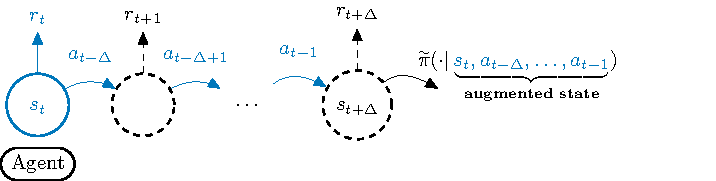
\includegraphics[bylabel=randomdelay]{img/thesis_plots.pdf}
    \caption{随机延迟示例：在时刻 $t$，延迟为 $n$；在时刻 $t+1$，延迟变为 $n'=n-1$。
    这意味着智能体观测到了 2 个新状态。
    步数之间的观测数量随机变量 $O$ 的概率定义为如\Cref{eq:observed} 所示概率的乘积。
    注意，索引 $t-n+1$ 的状态是否被观测到无关紧要，因为已观测到更近期的状态。}
    \label{fig:random_delay}
\end{figure}


该过程的奖励可定义如下，
\begin{align*}
    \augmentedexpectedrewardfunction(x,a) = \sum_{k=0}^{n}\probability(O=k)\sum_{i=0}^{k-1} \gamma^i\expectedvalue_{s_i\sim p^i(s_i\vert x,a)}[r(s_i,a_i)].
\end{align*}
该奖励基本上将新观测到的所有步数的奖励求和。
该定义假设，每当某个状态被观测到时，所有尚未观测到的中间状态将被同时观测到。

显然，涉及增广状态的过程定义了一个 \gls{mdp}，并证明了以下命题。

\begin{prop}
\label{pp:stoch_dmdp_is_mdp}
    具有独立同分布延迟 $(\delay_t)_{t\ge0}$（离散分布 $\zeta$，如上定义）的 \gls{dmdp} 可通过用最近的 $\delaymax$ 个动作和当前有效延迟增广状态来归结为 \gls{mdp}。
\end{prop}
该命题也在 \cite{bouteiller2020reinforcement} 中针对更一般的状态观测和动作执行延迟设定中被发现。
需要注意的是，包含动作执行延迟会带来一个问题：在给定时间步可能没有动作被执行，或者多个动作在同一时间步被执行。
在这些情况下，必须定义环境的行为。

现在考虑在此框架中应用 DIDA 学习的策略 $\delayedpolicy$，以研究当真实环境具有随机延迟但错误假设为常值延迟时的影响。
注意，DIDA 训练的常值 $\delay$-延迟 \gls{dmdp} 可视为上述过程的一个实例，其中 $\zeta$ 分布的全部权重放置在 $\delay$ 处。
在这种情况下，对于 $x = (s,a_1,\dots,a_\delaymax,n)$，认为 $\delayedpolicy(\cdot\vert x) = \delayedpolicy(\cdot\vert s,a_{\delaymax-\delay+1},\dots,a_\delaymax)$。
实际上，DIDA 将状态 $s$ 视为延迟了 $\delay$，并且对 $n$ 不可见。
将 DIDA 与如下定义的策略 $\widecheck{\pi}$ 进行比较：
\begin{align}
    \widecheck{\pi}(a\vert x) = \int_{\statespace} \augmentedbelief[n](s\vert x) \pi(a\vert s) \de s.\label{eq:belief_pol_stoch}
\end{align}
该策略的构造与 DIDA 相似，但适应 $n$ 的值。
下文中，记 $\widebar\delay$ 为随机延迟过程的平均延迟，定义如下：
\begin{align*}
    \widebar\delay = \expectedvalue[n] =  \sum_{k=0}^{\delaymax}k\prod_{i=0}^{k-1}\probability(\delay_i>i)\probability(\delay_k=k)
\end{align*}


\begin{thm}
\label{thm:stoch_mdp_dida_bound}
    考虑如上定义的具有随机延迟的 \gls{dmdp}，假设底层 \gls{mdp} 是 $L_T$-TLC 的。
    考虑由 DIDA 针对常值延迟学习的策略 $\delayedpolicy$（\Cref{eq:belief_pol}）和策略 $\widecheck\pi$（\Cref{eq:belief_pol_stoch}）。
    假设 $\delayedpolicy$ 的 Q 函数 $Q^\delayedpolicy$ 在第二个参数上是 $L_{\widetilde Q}$-LC 的\footnote{例如，当 $\gamma\max(L_P,1)\cdot(1+2L_\pi L_P)<1$ 时成立。该结果通过将 \cite[Theorem~1]{rachelson2010locality} 应用于常值延迟 \gls{mdp}（\Cref{pp:lip_dmdp}）和 DIDA 策略（\Cref{pp:lip_dida_pol}）的 Lipschitz 常数得到。}。
    则 $\delayedpolicy$ 和 $\widecheck\pi$ 之间的性能差异可界为：
    \begin{align*}
        \lvert V^{\widecheck{\pi}}(x)- V^{\delayedpolicy}(x)\rvert \le \frac{L_{\widetilde Q} L_\pi L_T }{1-\gamma}(\widebar\delay+\delay).
    \end{align*}
\end{thm}
\begin{proof}
    由\Cref{pp:stoch_dmdp_is_mdp}，随机延迟 \gls{dmdp} 是一个 \gls{mdp}。因此，可应用常规性能差异引理，对于 $x\in\widecheck{\augmentedstatespace}$\footnote{注意，本证明中，重载了原先定义于常值延迟 \gls{dmdp} 空间 $\augmentedstatespace$ 上的符号 $\delayeddiscountedstateoccupancydistribution[x][\delayedpolicy]$，改用空间 $\widecheck\augmentedstatespace$ 作为其定义域。}，
    \begin{align*}
        V^{\widecheck{\pi}}(x)- V^{\delayedpolicy}(x)
        = \frac{1}{1-\gamma} \expectedvalue_{x'\sim \delayeddiscountedstateoccupancydistribution[x][\widecheck\pi]} \left[\underbrace{V^{\delayedpolicy}(x) -  \expectedvalue_{a\sim \widecheck\pi(\cdot\vert x')}[Q^{\delayedpolicy}(x,a)]}_{A(x')}\right].
    \end{align*}
    如\Cref{th:perf_diff_bound} 中，可通过应用\Cref{pp:expected_q_bound} 推导以下界，其中记 $x'=(s',a_1',\dots,a_\delaymax',n')$，
    \begin{align}
        A(x')
        &\leq L_{\widetilde Q} \wassersteindistance(\widecheck\pi(\cdot\vert x')
        \Vert \delayedpolicy(\cdot\vert x'))
        \nonumber\\
        &= L_{\widetilde Q} \sup_{\left\Vert f\right\Vert_L\leq 1}\left\vert\int_{\actionspace} f(a)(\widecheck\pi(a\vert x')-\delayedpolicy(a\vert x') \de a\right\vert
        \nonumber\\
        &= L_{\widetilde Q} \sup_{\left\Vert f\right\Vert_L\leq 1}\left\vert\int_{\actionspace}\int_{\statespace} f(a)\pi(a\vert s)(\augmentedbelief[n'](s\vert x')-\augmentedbelief(s\vert x'))\de s  \de a\right\vert
        \nonumber\\
        &\leq L_{\widetilde Q} L_\pi \wassersteindistance(\augmentedbelief[n'](\cdot\vert x')
        \Vert \augmentedbelief(\cdot\vert x'))
        \nonumber\\
        &\leq L_{\widetilde Q} L_\pi L_T (n'+\delay),\label{eq:l_t_lip}
    \end{align}
    其中设定 $\augmentedbelief(s\vert x')=\augmentedbelief(s\vert s',a_1',\dots,a_\delaymax')$。这里使用了无延迟策略 $\pi$ 是 $L_{\pi}$-LC 的事实，\Cref{eq:l_t_lip} 通过复现\Cref{lem:bound_sigma_tlc} 的证明得到。
    因此，
    \begin{align*}
        V^{\widecheck{\pi}}(x)- V^{\delayedpolicy}(x)
        &\leq \frac{L_Q L_\pi L_T }{1-\gamma} \left(\delay +\expectedvalue_{x'\sim \delayeddiscountedstateoccupancydistribution[x][\widecheck\pi]}[n']\right)
        \\
        &= \frac{L_Q L_\pi L_T }{1-\gamma} \left(\delay +\widebar\delay\right),
    \end{align*}
    其中最后等式通过对增广状态中除 $n'$ 外的项积分得到。
\end{proof}

注意时间 Lipschitz 性质在证明中的重要性。
没有这一假设，$\wassersteindistance(\augmentedbelief[n'](\cdot\vert x')\Vert \augmentedbelief(\cdot\vert x'))$ 对 $x'$ 的依赖关系仍然存在，其在 $\delayeddiscountedstateoccupancydistribution[x][\widecheck\pi]$ 下的期望也不明确。
$n$ 与增广状态中其他元素之间确实存在非平凡依赖关系。
例如，当延迟较小时，$\statespace$ 中的某些状态可能被更频繁地访问。
另外注意，\Cref{th:perf_diff_bound} 中 $\statespace\subseteq\realnumbers^n$ 配备欧几里得范数的假设在此帮助不大，因为 $\wassersteindistance(\augmentedbelief[n'](\cdot\vert x')\Vert \augmentedbelief(\cdot\vert x'))$ 可能比较不同长度的轨迹（$n'\neq\delay$）。
DIDA 在该框架中对真实延迟不可见，构成了匿名延迟（anonymous delay）的情形（见\Cref{subsec:anonymous_delay_related}）。
据本文所知，这是 \gls{rl} 中匿名状态观测延迟的首个结果。
